\documentclass[a4paper]{article}
\usepackage{amsmath}
\usepackage{amsthm}
\newtheorem{thm}{Theorem}
\usepackage[english]{babel}
\usepackage[utf8]{inputenc}
\usepackage{graphicx}
\usepackage[colorinlistoftodos]{todonotes}
\setlength\parindent{0pt}
\usepackage[margin=0.7in]{geometry}
\usepackage{xspace}

\title{Omnet Router Specification}

\newcommand{\TU}{transaction unit\xspace}
\newcommand{\vls}[1]{{\color{blue} \textbf{Vibhaa:} {#1}}}
\newcommand{\TUs}{transaction units\xspace}
\newcommand{\NewPara}[1]{\noindent{\bf #1}}

%\author{Vibhaa Sivaraman}

\date{\today}
\begin{document}
\maketitle

\section{Transaction Unit}
Each \TU is a small amount of payment that is to be sent from one end-point to another. The route for a \TU is pre-specified by the sending end-point.
Thus, each \TU contains 6 fields: amount, time sent, sender, receiver, route, priority class. A \TU should never have an amount that is larger than a pre-defined {\em{Maximum Transaction Unit}}.
The route should have the sender and the receiver as the first and last entries. For starters, we don't assume deadlines on the completion of a \TU. As and when that is added, that 
can be added as a field. \vls{Add deadlines/priority explanation}

\section{Flow of Transaction Units - Simplistic Model}
\subsection{Overview}
The high level flow per transaction unit is as follows. Let's consider a transaction arriving at router $A$ and meant to be sent out on the $A-B$ channel. When a \TU is received at 
$A$ whose next hop is $B$, we first check if there is already a queue of \TUs waiting to be sent out to $B$. If so, we add this new \TU (let's say $t$) to it. If not, we check 
if there were sufficient funds available to send out $t$. If not, we add $t$ to the queue and are done for this transaction unit. If there are funds available, 
we update the balances (decrement) on $A$'s end for the $A-B$ channel. When $B$ receives the same \TU, it increments its balance on the $A-B$ channel. Note that this naturally introduces a delay
in the balance update because of ``propagation delay'' of the \TU. If this balance increment frees up any funds for further \TUs currently queued at $B$, they should be sent out on the $B-A$ channel.

Once $B$ has completed the updates for the $A-B$ channel for the original \TU $t$, it looks at the next hop and repeats the procedure on the outgoing channel at $B$.

This is illustrated in the following flowchart.
\begin{figure}[h]
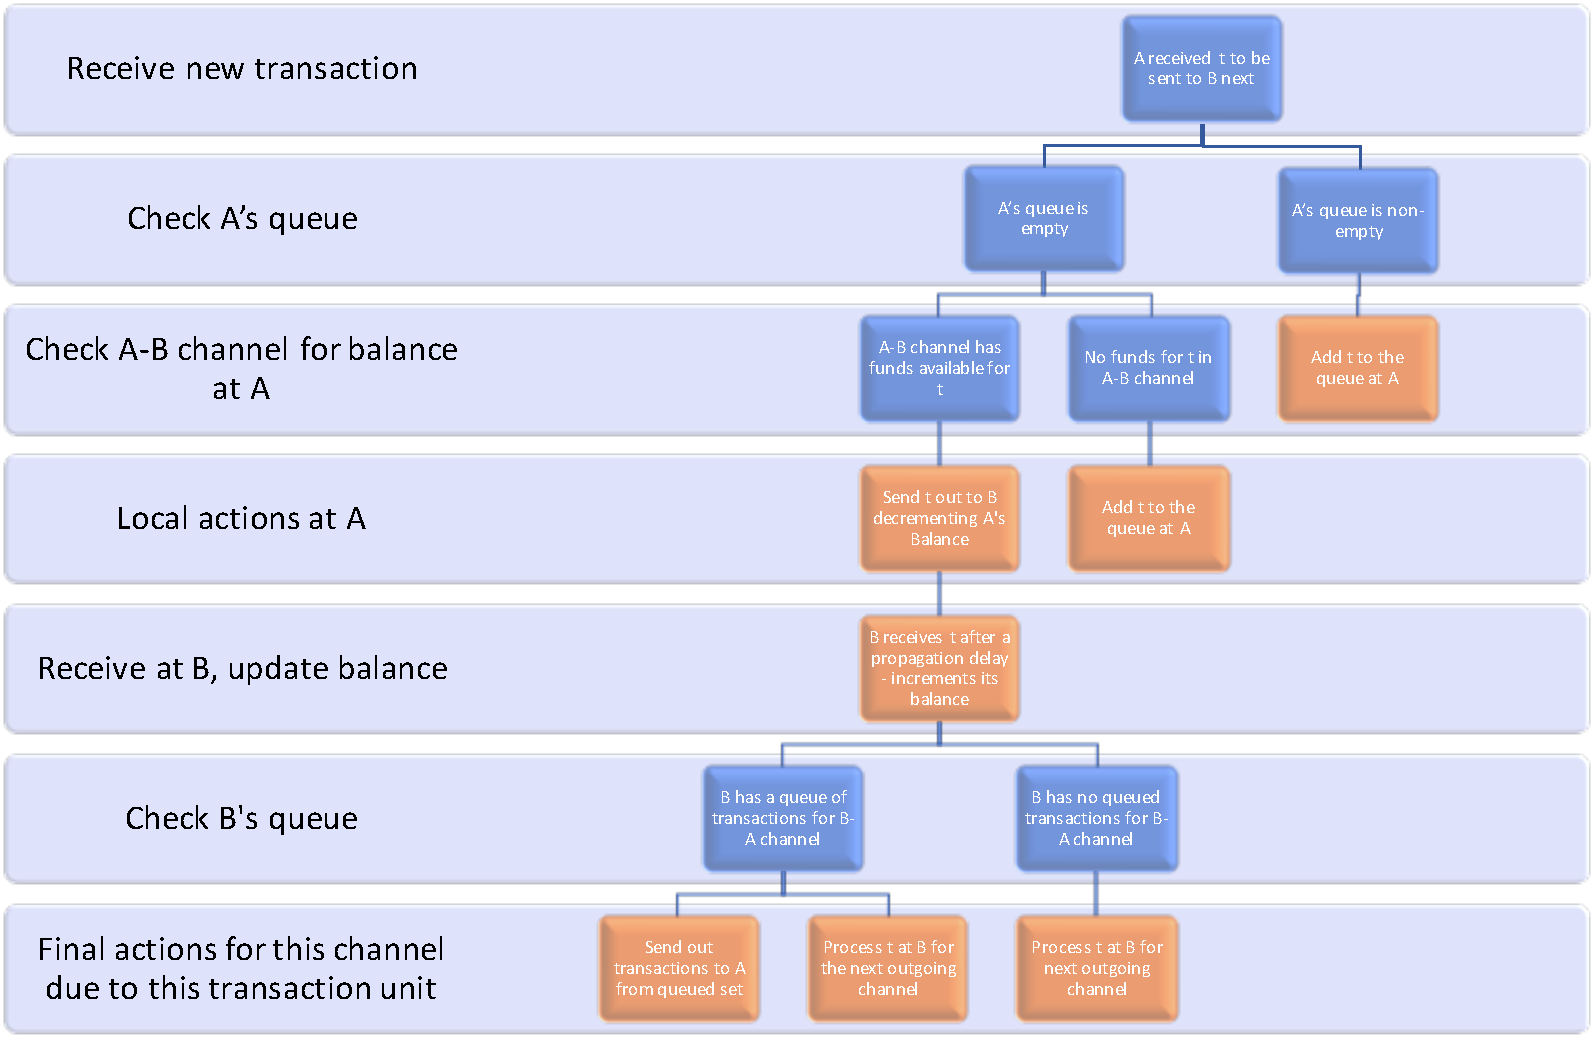
\includegraphics[width=\linewidth,height=10cm]{router_flow.pdf}
\caption{flow of transactions at a router}
\label{fig:routerflow}
\end{figure}

\subsection{Message Types}
We only have one message corresponding to a \TU.
\begin{itemize}
            \item Amount
            \item Time sent
            \item Original Sender
            \item Receiver
            \item Route
            \item Priority Class

\end{itemize}

\subsection{State Per Router}
This necessiates the following states at a router and the ability to update them
\begin{itemize}
    \item Router state (Map to identify channels): key is neighboring router id (typically public key) and value is a unique channel index or id. 
        The idea is that you would use this to identify the channel id when you have the route of a packet in terms of hops/routers it traverses. Once you have this id,
        you can use it to index into a table that contains every channel's state (described below).
    \item Per channel state:
        \begin{itemize}
            \item Balance for oneself and for the other party
            \item Queue of \TUs (in the above example, it would be a queue at A of \TUs it wanted to send to B but didn't have funds for)
      \end{itemize}
\end{itemize}


\subsection{Event Handlers for a Single Router}
This follows from the flowchart above. 
\begin{itemize}
    \item Receipt of a transaction $t$: 
        \begin{itemize}
            \item Increment balance for self by t.amount on the incoming channel
            \item Check if any transactions were queued for the incoming channel (in the opposite direction) that can now be sent out because of the increment in balance
            \item Send as many as you can in priority order on that incoming channel
        \end{itemize}
    \item Process transaction $t$:
        \begin{itemize}
            \item Inspect next hop for $t$, map it to right outgoing channel id using the channel - channel id map per router
            \item Check if there's already transactions queued for that channel in the per channel queue
            \item If there's already queue just add $t$ to the queue for the outgoing channel
            \item If there isn't a queue, check if we have sufficient funds for $t$. If not, again, queue $t$
        \end{itemize}
    \item Send transaction $t$:
        \begin{itemize}
            \item Decrement balance for outgoing channel
            \item Send message on the outgoing channel (assume some propagation delay after which it will be received there)
        \end{itemize}
\end{itemize}








\section{Flow of HTLCs - With Receiver Acknowledgements}
\subsection{Overview}
\NewPara{Sending out HTLCs} The high level flow per HTLC is as follows. Let's consider a HTLC arriving at router $A$ and meant to be sent out on the $A-B$ channel. When a HTLC is received at 
$A$ whose next hop is $B$, we first check if there is already a queue of HTLCs waiting to be sent out to $B$. If so, we add this new HTLC (let's say $t$) to it. If not, we check 
if there were sufficient funds available to send out $t$. If not, we add $t$ to the queue and are done for this HTLC for now. If there are funds available, 
we update the balances (decrement) on $A$'s end for the $A-B$ channel. So far, this is similar to the previous simplistic model. 

However, while this means that the HTLC has been attempted on this channel and is going out from $A$ to $B$, it hasn't been cleared yet. So, we add $t$ to a set of the inflight
outgoing HTLCs which represents the set of HTLCs that have been attempted but not cleared yet. When $B$ receives the same HTLC, it adds $t$ to a set of inflight incoming HTLCs 
(that have been received but haven't been cleared yet). Note that this naturally introduces a delay in adding $t$ to the HTLCs at $B$.
This is because of ``propagation delay'' of the HTLC. During this time, the total capacity of the channel is a little less than the original capacity because only one node knows
about the HTLC $t$ (roughly similar to before). Once $B$ has completed this, it looks at the next hop and repeats the procedure on the outgoing channel at $B$. $B$ does nothing further
on the $A-B$ channel for this HTLC until an {\em{ack}} is received.

\bigskip

\NewPara{Responding to Successful Acks} Now, once the HTLC has been received at the destination node, this node will relay a successful {\em{ack}} backwards along the route of the transaction which will effectively clear 
the transactions from the ``inflight HTLC'' queues on individual routers for each channel. For instance, when $B$ receives a successful ack for some HTLC
$t$ from a neighbor node $C$, it must first remove $t$ from the set of inflight outgone HTLCs. It doesn't need to update
any balance information since the balance was already decremented. $B$ sends a balance update to $C$ to tell $C$ that it has reliably decremented the balance. ($C$ can now remove $t$ from its incoming pending HTLCs and 
increment its balance accordingly).
$B$ sends the ack to $A$ which sent the HTLC in the first place to $B$. Once it has received a balance update from $A$ for transaction $t$, $B$ clears $t$ from
the set of inflight incoming HTLCs and increments its view of the $A-B$ balance accordingly.

\bigskip

\NewPara{Failure Acks} (Can wait on this) Now, once a given node has decided to fail an HTLC, it can relay a failure {\em{ack}} backwards along the route of the transaction which will effectively clear 
the transactions from the ``inflight HTLC'' queues on individual routers for each channel all the way up. For instance, when $B$ receives a failure ack for some HTLC
$t$ from a neighbor node $C$, it must first remove $t$ from the set of inflight outgone HTLCs. It also needs to update its balance information since the balance was already decremented. 
$B$ sends the ack to $A$ which sent the HTLC in the first place to $B$. $B$ also clears $t$ from
the set of inflight incoming HTLCs since it can't complete.


This is illustrated in the following flowchart.
\begin{figure}[h]
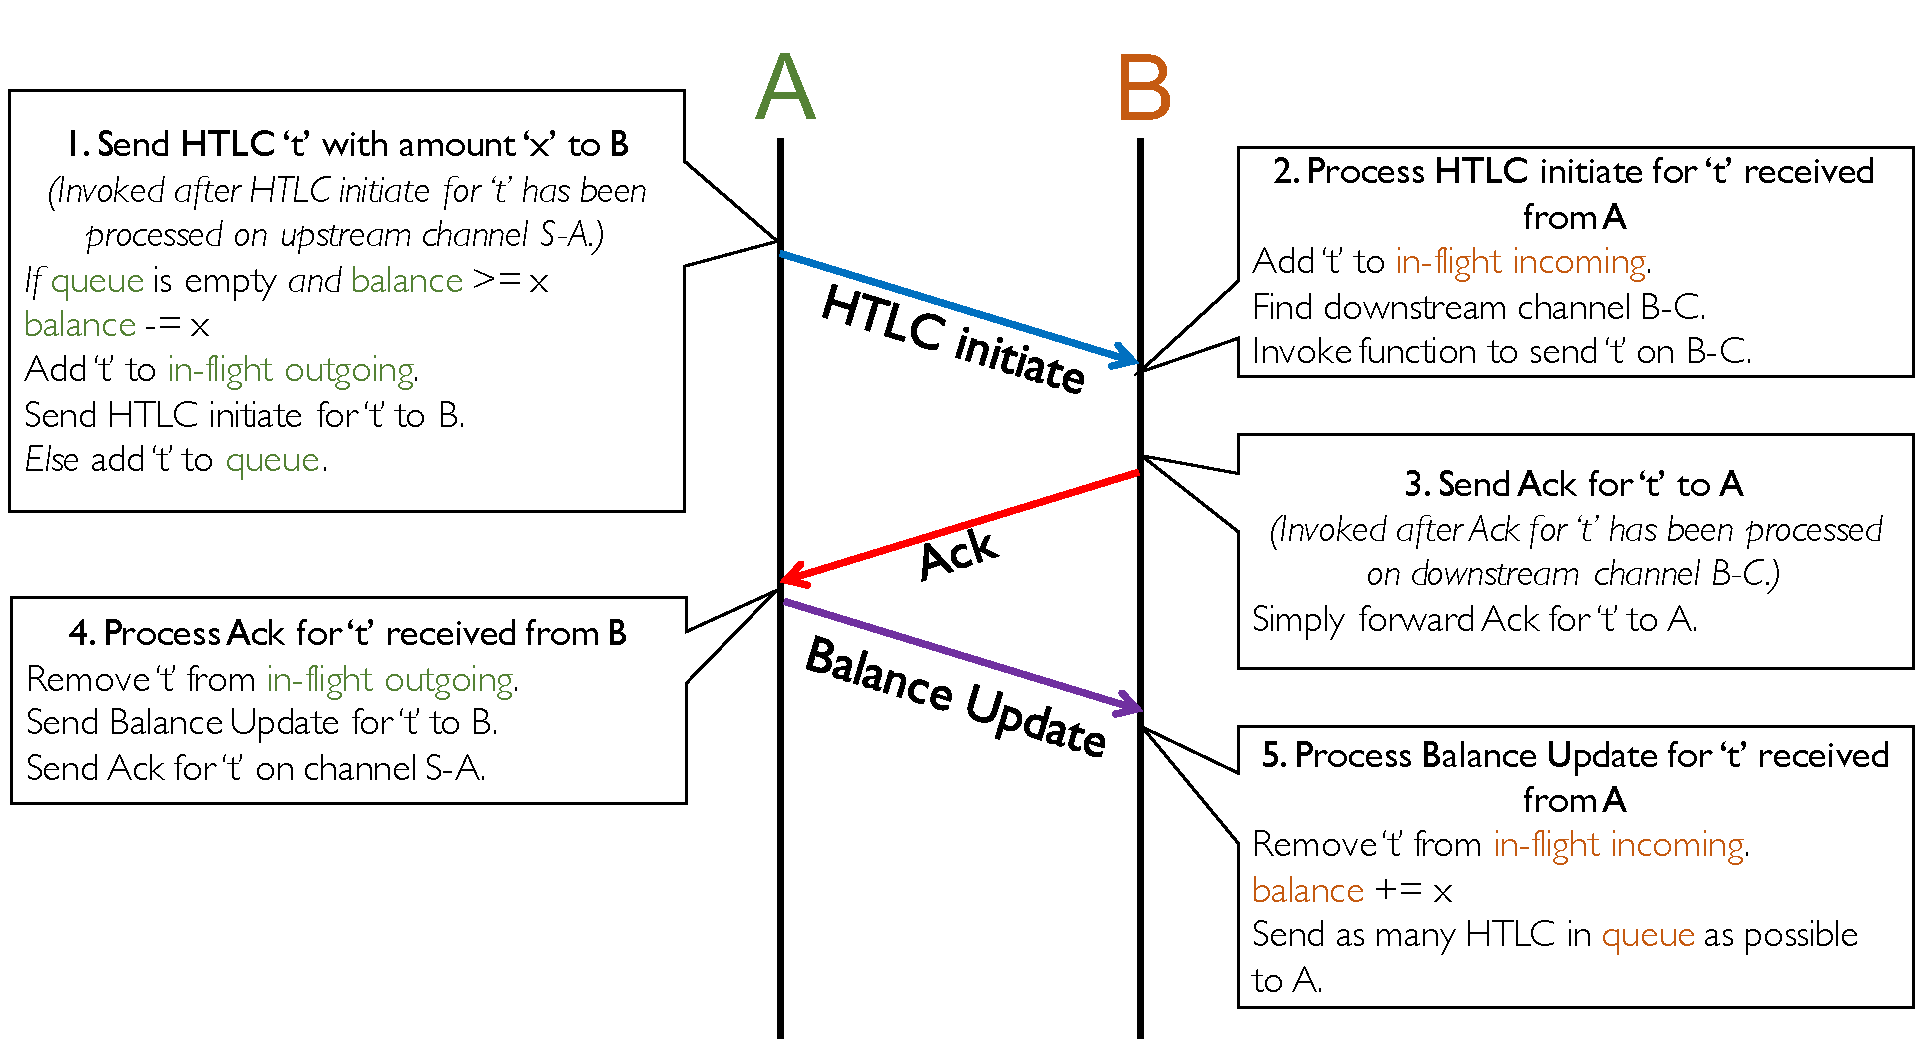
\includegraphics[width=\linewidth,height=10cm]{htlcAckFlow.pdf}
\caption{flow for a given HTLC $t$ at a given channel}
\label{fig:htlcflow}
\end{figure}


\subsection{Message Types}
\begin{itemize}
    \item HTLC Initiate: This is similar to the current transaction message
        \begin{itemize}
            \item Amount
            \item Time sent
            \item Original Sender
            \item Receiver
            \item Route
            \item Priority Class
            \item Transaction id (needed for removing it from the set of inflight transactions)
        \end{itemize}

    \item HTLC Ack
        \begin{itemize}
            \item Transaction id for which the Ack is received
            \item Route for the ack (reverse of the path the transaction was sent on
            \item Status (Success or Failure) - just in case we want to simulate failures and propagate them upwards
            \item Secret - Dummy field for now (might never change)
        \end{itemize}

    \item Balance Update
        \begin{itemize}
            \item Transaction id that is being completed (Assuming that the inflight transaction set at each node has the amount already, this is all we really need to update the balances correctly)
            \item Local Balance (The one who is sending the message)
            \item Other Party's balance (the one the message is sent to)
        \end{itemize}
\end{itemize}

\subsection{State Per Router}
This necessiates the following states at a router and the ability to update them
\begin{itemize}
    \item Router state (Map to identify channels): key is neighboring router id (typically public key) and value is a unique channel index or id. 
        The idea is that you would use this to identify the channel id when you have the route of a packet in terms of hops/routers it traverses. Once you have this id,
        you can use it to index into a table that contains every channel's state (described below).
    \item Per channel state:
        \begin{itemize}
            \item Balance for oneself and for the other party
            \item Queue of \TUs (in the above example, it would be a queue at A of \TUs it wanted to send to B but didn't have funds for)
            \item Inflight transactions that were sent out on this channel - hashmap with transaction ids as keys and amount as value
            \item Inflight transactions that came into this channel - hashmap with transaction ids as keys and amount as value
        \end{itemize}
\end{itemize}

\subsection{Event Handlers for a single Router}
This follows from the flowchart above. 
\begin{itemize}
    \item Receipt of an incoming incomplete HTLC $t$ from upstream router: 
        \begin{itemize}
            \item Add $t$ and the amount to incoming inflight transaction set
             \item Process HTLC $t$:
                \begin{itemize}
                    \item Inspect next hop for $t$, map it to right outgoing channel id using the channel - channel id map per router
                    \item Check if there's already transactions queued for that channel in the per channel queue
                    \item If there's already queue just add $t$ to the queue for the outgoing channel
                    \item If there isn't a queue, check if we have sufficient funds for $t$. If not, again, queue $t$
                \end{itemize}
            \item Send HTLC $t$ to downstream router:
                \begin{itemize}
                    \item Decrement balance for outgoing channel
                    \item Add $t$ and the amount to outgoing inflight transaction set
                    \item Send ``HTLC Initiate'' message on the outgoing channel (assume some propagation delay after which it will be received there)
                \end{itemize}
        \end{itemize}
    \item Receive HTLC $t$'s ack from downstream router:
        \begin{itemize}
            \item Successful ack:
                \begin{itemize}
                    \item Remove $t$ from outgoing inflight transaction set on (me - downstream) router channel
                    \item Send ``balance update'' message to the downstream router with your own balance decremented and the other router's incremented
                    \item Send ``HTLC ack'' to upstream router
                \end{itemize}
            \item Failure Ack:
                \begin{itemize}
                    \item Remove $t$ from outgoing inflight transaction set and increment my side of the balance
                    \item Send ``Failure HTLC ack'' to upstream router
                    \item Remove $t$ from incoming inflight transaction set for the corresponding channel it came in on
                \end{itemize}

        \end{itemize}
    \item Receipt of balance update
        \begin{itemize}
            \item Increment my side of the balance by the corresponding amount
            \item Check if any transactions were queued for the incoming channel (in the opposite direction) that can now be sent out because of the increment in balance
            \item Send as many as you can in priority order on that incoming channel

        \end{itemize}
\end{itemize}

\end{document}


